\chapter{肢 痛}

肢痛疾病的分类见表\ref{tab45-1}。

\begin{longtable}{c}
 \caption{肢痛疾病的分类}
 \label{tab45-1}
 \endfirsthead
 \caption[]{肢痛疾病的分类}
 \endhead
 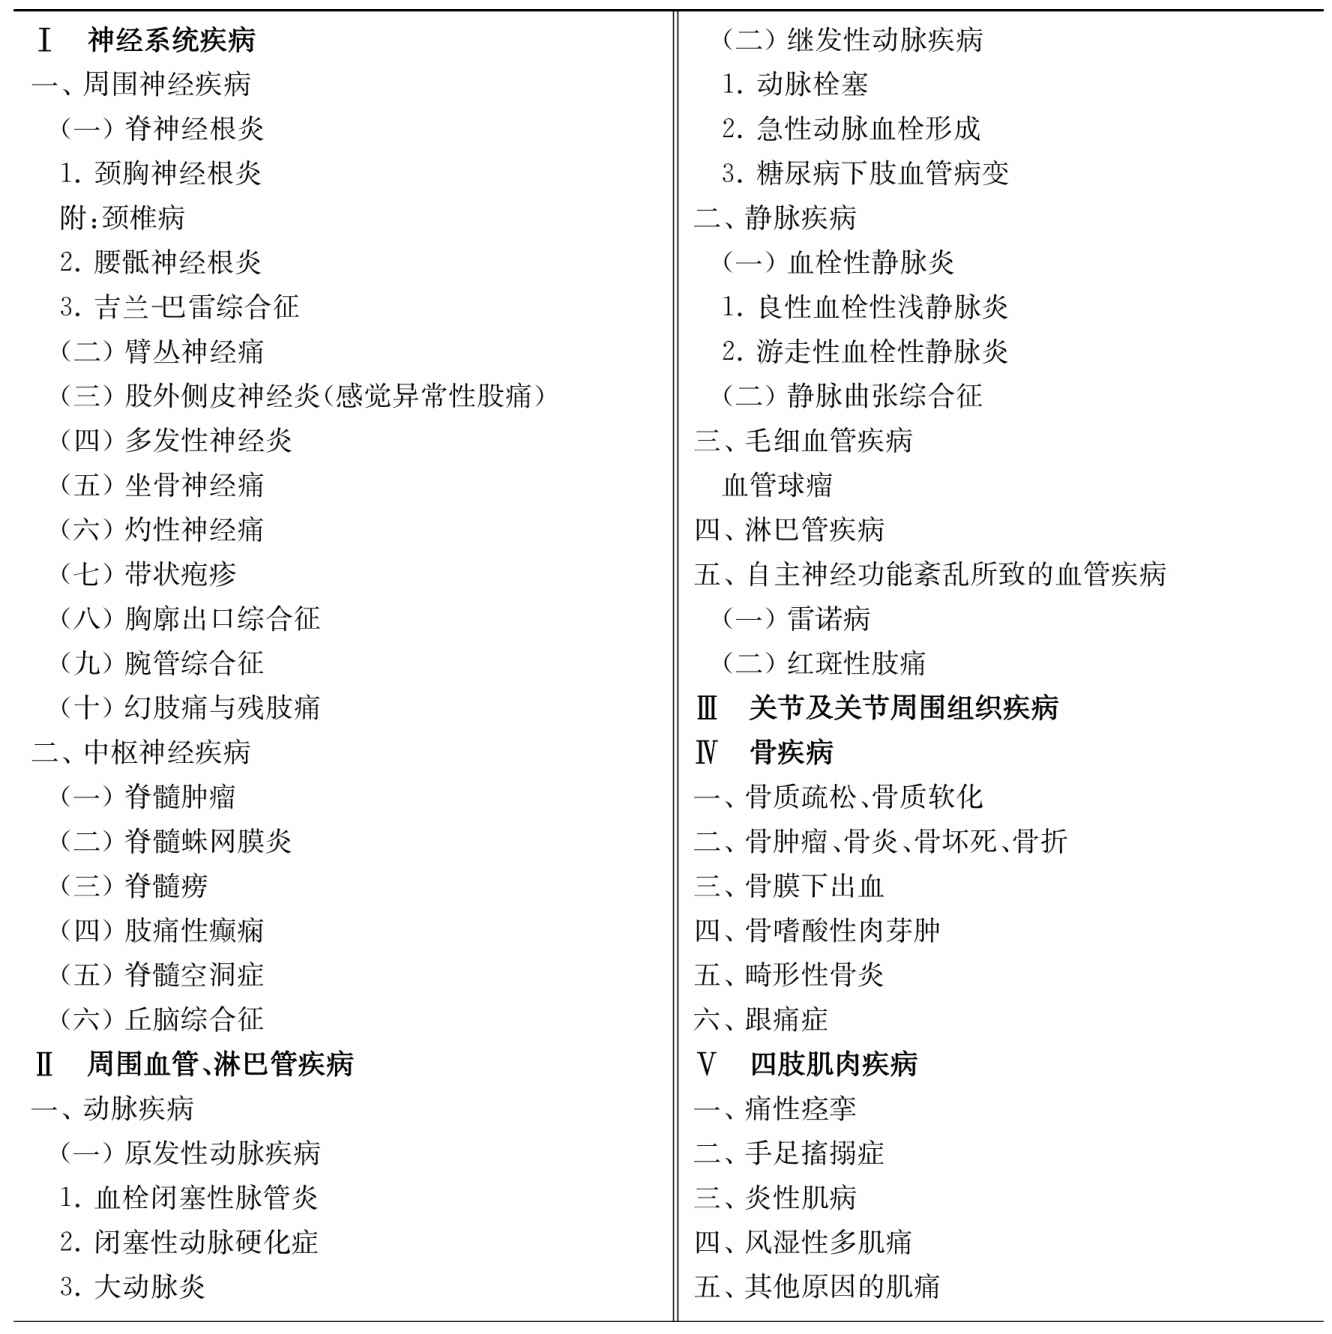
\includegraphics[width=\textwidth,height=\textheight,keepaspectratio]{./images/Image00272.jpg}\\
 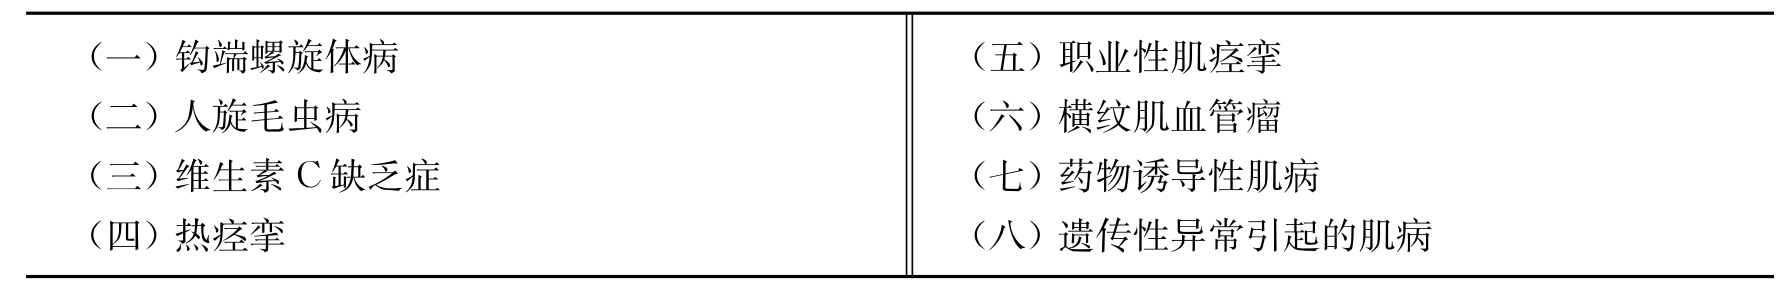
\includegraphics[width=\textwidth,height=\textheight,keepaspectratio]{./images/Image00273.jpg}
 \end{longtable}

肢痛作为一种常见的临床症状,其病因众多,四肢的皮肤、皮下脂肪组织、肌肉、骨、关节、血管、淋巴管、神经、筋膜、韧带、肌腱、腱鞘、滑囊等病变(如炎症、肿胀、肌肉缺血等所致的痛觉感受器刺激)均可引起。导致肢痛的常见疾病有下列几方面(参见表\ref{tab45-1})。

1.神经系统病变%}

由于机体的感觉神经纤维和自主神经受到病变刺激,往往发生不同程度的疼痛,最常见的有周围神经炎、外伤和受压,其次为脊髓病变所致的神经根受刺激。

2.周围血管、淋巴管病变%}

由于四肢动脉管腔狭窄、阻塞,皮肤或皮下组织血管收缩和舒张的功能紊乱,均可导致肢体血液循环不足而产生缺血性疼痛,如血栓闭塞性脉管炎、闭塞性动脉硬化症、雷诺病、动脉栓塞和红斑性肢痛等。此外,血栓性静脉炎、静脉曲张也可导致肢体疼痛。

3.关节及关节周围组织病变%}

四肢关节急性或慢性炎症,不论休息或活动时,患者均可感到自发性疼痛,如病变在小关节上,则可发生刺痛和麻木感。常见的有类风湿关节炎、骨关节炎等。

4.骨病变%}

常见的有骨质疏松、骨髓炎、骨结核、骨肿瘤、无菌性骨坏死等。

5.四肢肌肉病变%}

引起肌肉疼痛的原因主要是肌肉痉挛如手足搐搦症;肌肉缺氧时,中间代谢产物如乳酸及丙酮酸积聚也可产生肌肉疼痛。

肢痛病因的诊断,首先需注意病史与体格检查。病史中如年龄、性别、个人嗜好可有参考价值,如雷诺病多见于年轻女性,血栓闭塞性脉管炎多见于20~40岁吸烟的男性,闭塞性动脉硬化症往往发生于60岁以上的老年人等等。体检时注意双侧肢体是否对称,有无溃疡或坏疽,两侧肢体的肤色、皮温、感觉、肌力、肿胀、动脉搏动等方面有无差异。准确的神经系统检查对神经系统疾病的诊断帮助很大。怀疑为脊髓痨的患者需检查有无阿罗(Argyll-Robertson)瞳孔、膝反射。

在分析肢痛的病因时,首先需区别是血管性或非血管性病变所引起。通过详细的病史询问,一般可以初步确定是血管性或非血管性;应了解肢痛的部位,是单侧或双侧、上肢或下肢、起病因素、有何伴随症状等。血管性病变的肢痛多有皮肤颜色、温度的改变,疼痛发作与运动、休息、体位、药物、外界温度和湿度有密切关系。典型的雷诺病,双手受寒冷刺激时,则发生动脉痉挛性痛和皮色变白;红斑性肢痛时,双足遇热或下垂时,往往引起疼痛加剧,抬高患肢或局部冷敷则疼痛缓解。如突然发生的肢体剧烈疼痛、感觉异常、运动消失、肢体皮肤苍白,常提示动脉急性栓塞。当出现间歇性跛行时,则提示下肢动脉供血不足,需注意血栓闭塞性脉管炎和闭塞性动脉硬化症等情况。间歇性跛行伴有静止痛,说明血管功能严重损害;若仅有剧烈的静止痛而不伴有间歇性跛行,则肢痛可能为非血管性病变所致,还需进一步鉴别是由其他何种原因(如神经、肌肉、骨或关节病变)所致。神经系统病变引起的肢痛,其疼痛多沿罹患神经分布或放射,常同时伴有其他神经系统症状。如腰神经根第4、5和骶神经根第1、2、3部位病变引起的下肢痛,是从腰部向臀部、大腿后侧及小腿后外侧和踝部放射。肌肉病变引起的肢痛,主要表现为受累肌肉有自发性酸痛或剧痛,局部有触痛和压痛,可伴肌肉萎缩和肌力减退。肌肉痉挛性疼痛可在夜间突然发作,常表现为小腿剧痛,持续数分钟,经肌肉按摩及活动后可缓解。关节和骨病变引起的疼痛,部位明确固定,疼痛呈持续性,按压病变处疼痛加剧,伴关节肿胀和功能障碍。

实验室与影像学检查对肢痛原因的分析具有重要价值,有时甚至起到决定性的作用,但其结果不能孤立地看待,要注意与临床表现相结合。实验室检查方面,除血、尿常规外,应根据诊断思路尽可能地完善相关检查,如考虑可能存在自身免疫性疾病应进行全面的免疫血清学检查,对中枢神经系统病变还应考虑作脑脊液检查。脊椎、上、下肢、骨关节病时作X线、磁共振等影像学检查,对确定诊断往往有较大帮助。

\protect\hypertarget{text00339.html}{}{}

\section{149 神经系统疾病}

\subsection{一、周围神经疾病}

\subsubsection{(一)脊神经根炎}

脊神经根炎是指脊髓前根和后根(位于脊膜腔内)病变,疼痛的特点是沿神经根分布区的刺激性放射性疼痛,体检常在相应的脊椎棘突或棘突旁有压痛;在引起脑脊液压力增高的情况下,如咳嗽、喷嚏、震动或用力排便时,疼痛往往加剧。当低头或弯腰等动作使神经根受牵拉时,疼痛也加剧。病变严重时可有肢体无力、腱反射减弱与轻度肌萎缩。脑脊液检查多有蛋白量增加,少数病例蛋白量与细胞数两者均有增加。

引起四肢痛的脊神经根炎如下文所述。

\paragraph{1.颈胸神经根炎}

本病发病年龄往往较轻,常由病毒感染所致,发病前多有上呼吸道感染史。主要症状为一侧或双侧颈、上胸、背、肩、臂部或直到肘、腕、指部放射性疼痛或麻木感。疼痛时轻时重,性质为酸痛、钝痛,也可为刀割样痛。患肢可有感觉减退、运动障碍,腱反射减弱或消失。当头颈部或患肢作过度伸屈运动时,疼痛往往加剧。

颈胸神经根炎、颈椎病、肩手综合征等易互相混淆。神经根型颈椎病可出现颈部、肩部和一侧上肢疼痛,颈部僵硬、活动受限,常有明确的压痛点伴放射性疼痛,同时伴有上肢的感觉和运动功能障碍。脊髓型颈椎病也可出现与神经根型相似的上肢症状,但多无颈部疼痛和感觉障碍。肩手综合征则包括各种原因所致的上肢神经营养障碍。

本病还需与纤维肌痛综合征、肩关节周围炎、脊髓病变(尤其是肿瘤、蛛网膜炎)早期引起的神经根刺激症状、颈椎结核等相鉴别。纤维肌痛综合征有睡眠障碍和特异的压痛点,无感觉障碍。肩关节周围炎主要表现为肩关节外展旋转障碍与疼痛,神经系统检查无异常。脊髓病变早期引起的神经根刺激症状,常局限于1~2个神经根的损害,必要时可作脑脊液检查与脊髓MRI检查,以明确诊断。颈椎间盘脱出则有明确的外伤史,起病急,疼痛剧烈,X线摄片有助于诊断。颈胸椎结核的发病年龄较轻,可根据放射学检查所见而与本病鉴别。

上述一系列颈神经根受压症状,其由颈椎病、颈肌损伤、颈肌炎症等引起者,也有人称为颈神经根综合征。

颈椎病以男性罹患较多,发病常在40岁以上,最常累及负重最大的5、6颈椎,其次为4、7颈椎。通常主诉为缓慢出现的单侧颈根和肩部疼痛,可向同侧上、下臂与手指放射,往往在夜间较剧。疼痛向上臂外侧放射者,提示为颈5神经根受累;疼痛向上臂外侧和前臂桡侧放射者,提示为颈6~7神经根受累;疼痛放射至前臂内侧和4、5指者,提示为颈3神经根受累。但颈椎病时往往累及多神经根。体检常于颈椎棘突或椎旁有压痛,头顶加压试验及颈神经根紧张试验(患侧肩下压,头向对侧推移)阳性,即患侧颈、肩及上肢发生疼痛。检查者用双手将患者头部向上牵引则疼痛减轻或消失。颈椎增生性变可经X线颈椎正、侧位平片检查而确定。

国内颈椎病专题座谈会曾制定颈椎病诊断标准,对颈椎病的定义为:颈椎椎间盘组织退行性变及其继发病理改变累及其周围组织结构(神经根、脊髓、椎动脉、交感神经等),出现相应的临床表现者称为颈椎病。一般原则:

(1)临床表现与影像学所见相符合者,可以确诊。

(2)具有典型颈椎病的临床表现,而影像学所见正常者,应注意除外其他疾患后方可诊断为颈椎病。

(3)仅有影像学表现异常,而无颈椎病临床症状者,不应诊断为颈椎病。

各型颈椎病的诊断标准:

\subparagraph{(1)颈型:}

①主诉头、颈、肩疼痛等感觉异常,并伴有相应的压痛点;②X线平片上颈椎显示曲度改变或椎间关节不稳等表现;③除外颈部其他疾患(落枕、肩周炎、纤维肌痛综合征、神经衰弱及其他非椎间盘退行性变所致的肩颈部疼痛)。

\subparagraph{(2)神经根型:}

①具有较典型的根性症状(麻木、疼痛),且范围与颈脊神经所支配的区域相一致;②压颈试验或臂丛牵拉试验阳性;③影像学所见与临床表现相符合;④痛点封闭无显效(诊断明确者可不做此试验);⑤除外颈椎外病变(胸廓出口综合征、网球肘、腕管综合征、肘管综合征、肩周炎、肱二头肌腱炎等)所致以上肢疼痛为主的疾患。

\subparagraph{(3)脊髓型:}

①临床上出现颈脊髓损害的表现;②X线平片上显示椎体后缘骨质增生、椎管狭窄,影像学证实存在脊髓压迫;③除外肌萎缩性脊髓侧索硬化症、脊髓肿瘤、脊髓损伤、继发性粘连性蛛网膜炎、多发性末梢神经炎。

\subparagraph{(4)椎动脉型:}

此型颈椎病的诊断问题尚待研究。①曾有猝倒发作,并伴有颈性眩晕;②旋颈试验阳性;③X线平片显示节段性不稳定或颈椎关节骨质增生;④多伴有交感症状;⑤除外耳源性、眼源性眩晕以及椎动脉Ⅰ、Ⅲ段受压引起的基底动脉供血不全。

\subparagraph{(5)交感神经型:}

临床表现为头晕、眼花、耳鸣、手麻、心动过速、心前区疼痛等一系列交感神经症状。X线片有失稳或退变,椎动脉造影阴性。

患者也可表现为混合型的症状。

\paragraph{2.腰骶神经根炎}

腰骶神经根炎常由于腰骶椎病变、劳损或感染所致,其疼痛在腰、骶和臀部并放射至下肢。临床表现主要为下背部痛和腰部僵直感,局部有明显压痛,直腿抬高试验(Laségue征)和Wasserman征(患者俯卧,检查者抬起其伸直的患腿,使股神经受牵拉时沿患腿前面股神经分布区域发生疼痛)均呈阳性,腰骶部及下肢活动受限制或呈保护性姿势;病变加重时,于腰骶部出现节段型感觉障碍、下肢无力、肌肉萎缩、腱反射减退。本病常需与单纯性骨关节病变、腰肌劳损及椎管内腰骶部病变(如马尾、圆锥肿瘤)所致的神经根刺激症状以及脊柱关节病相关的腰骶部和下肢疼痛相鉴别。X线检查易与单纯性骨关节病变区别。腰肌劳损主要表现为腰肌僵硬感和压痛,无神经系统体征。椎管内腰骶部病变引起神经根激惹症状,则往往需作脑脊液检查才能鉴别。此外,腰骶神经根炎如病变范围局限于腰4~5和骶1~3,其临床表现与根性坐骨神经痛相同,临床上很难区别。通过X线、MRI等影像学和HLA-B27等检查一般也不难与脊柱关节病(如强直性脊柱炎)鉴别。

\paragraph{3.吉兰-巴雷(Guillain-Barré)综合征}

本综合征又名急性感染性多发性神经根神经炎,四肢痛是本综合征早期的一个突出表现。患者于早期除常有不同程度的上呼吸道感染症状外,主要是四肢自发性痛,检查时患者甚至不能忍受。由于其周围神经受损害,故常伴随四肢无力、麻木、感觉减退或消失、腱反射减弱等,此外,患者也常有脑神经损害。脑脊液检查出现蛋白、细胞分离现象,即蛋白明显增高,而细胞数正常或轻度增高。

\subsubsection{(二)臂丛神经痛}

臂丛由第5、6、7、8颈神经根及第1胸神经根组成,其主要位置在锁骨上、下窝。臂丛的功能大部分是支配上肢,罹病时疼痛首先在胸颈根部和锁骨上部臂丛区,迅即扩展至肩后部,放射至臂和手。疼痛初期呈间歇性,但可迅速变为持续性而影响整个上肢,患者多呈屈肘姿势,并避免不必要的运动以减轻疼痛。睡眠时不敢取病侧侧卧位,锁骨上窝及神经干有压痛,牵引上肢向外后上方活动时疼痛加剧。此外患侧上肢无力、麻木和腱反射减弱,常与肩关节周围炎和颈胸神经根炎相混淆。肩关节周围炎的疼痛局限于肩部,无神经系统症状。臂丛神经痛与颈胸神经根炎的区别,可根据疼痛的主要部位及感觉障碍的类型。前者主要为锁骨上部臂丛区疼痛,皮肤感觉障碍多不明显,后者为颈椎下段、胸椎上段痛,常有节段型感觉减退。

臂丛损害的原因最常为感染、外伤(如颈部、锁骨上窝及肩部外伤)、锁骨骨折、头固定时臂部过度运动或臂固定时头部过度运动,以及难产时施行胎儿牵引手术等。

\subsubsection{(三)股外侧皮神经炎(感觉异常性股痛)}

股外侧皮神经发自腰丛,通过腹股沟韧带,距髂前上棘5~10cm处穿出大腿的阔筋膜,而分布于大腿前外方下2/3的部位。发病多为20~50岁的男性。发病原因可为感染、受冷、盆腔病变或神经受压。主要症状是大腿前外方下2/3感觉异常,以麻木最为多见;部分患者有疼痛(刺痛、灼痛),在行走或站立时疼痛加重。客观检查可发现相应部位的痛觉与温度觉减退,而触觉与压觉存在。本病国内曾有多例报告。

\subsubsection{(四)多发性神经炎}

多发性神经炎是指四肢远端末梢神经病变。发病早期的自觉症状为手指或足趾的疼痛或发麻。病变区的皮肤可有痛觉过敏现象,即轻触也可引起疼痛,感觉异常如蚁行感、刺痛等也常发生,伴肌肉压痛。此外,尚有四肢感觉、运动和自主神经营养障碍。

\subsubsection{(五)坐骨神经痛}

坐骨神经起自骶丛,即由第4、5腰神经根和第1、2、3骶神经根组成,先入骨盆,向下穿过梨状肌,分布于臀部,沿大腿后面下行,到达腘窝稍上处即分成腓总神经和胫神经。腓总神经向外向前分为腓深神经和腓浅神经,走至足背;胫神经则由腘窝一直沿小腿后面走至足底。在脊髓分出的近侧段为神经根部,在骶丛分出之后为神经干部。临床上根据其发病部位不同,区别为根性坐骨神经痛及干性坐骨神经痛。根性坐骨神经痛的临床表现与腰4~5骶1~3的神经根损害所表现的症状相同。以下主要介绍干性坐骨神经痛。

干性坐骨神经痛的特点主要为沿坐骨神经分布区疼痛。疼痛多呈持续性钝痛而有发作性加剧,发作性疼痛呈烧灼样和刀刺样性质,且常在夜间加剧,患者往往取一系列的减痛姿势。例如睡时取健侧卧位及微屈病侧下肢,从仰卧位起坐时即屈曲病侧膝关节;坐下时以健侧臀部先着力,站立时身体重心略向健侧倾斜,患者下肢在髋、膝关节处微屈,造成脊椎侧弯,凸部多朝向健侧。干性坐骨神经痛常有下列压痛点:①臀点:相当于环跳穴,在坐骨结节与股骨大粗隆之间;②腘点:腘窝线中点向上约2cm处;③腓肠肌点:在小腿后面的中央,相当于承山穴;④踝点:在外踝之后,相当于昆仑穴。90\%以上的患者直腿抬高试验阳性,此外,尚可见坐骨神经所支配的肌肉如后腘肌和腓肠肌等出现肌肉松弛和萎缩,跟腱反射减弱或消失,患肢小腿外侧和足背有感觉减退区。

临床上根性坐骨神经痛比干性坐骨神经痛多见,某些病例则两者同时存在,根据下述情况一般可将两者区别。根性坐骨神经痛于咳嗽、喷嚏和用力时疼痛加剧;腰椎棘突和横突压痛最为显著,Neri征阳性(于仰卧时屈颈或向前弯腰,患侧下肢即自动屈起,同时腰腿痛加剧,为阳性)和交叉性直腿抬高征阳性(将患者健侧腿抬高,患侧腿出现疼痛,为阳性);脑脊液中蛋白或细胞多有改变。干性坐骨神经痛以沿坐骨神经压痛点的压痛较明显,而无腰部体征,交叉性直腿抬高征常为阴性,脑脊液一般无改变。

根性坐骨神经痛最常见的病因是腰骶椎间盘脱出,其次为椎管内肿瘤压迫、腰骶神经根炎、脊髓腰段蛛网膜炎、脊椎关节炎等。干性坐骨神经痛多见于感染性坐骨神经炎、盆腔疾病和脊椎关节疾病等。

\subsubsection{(六)灼性神经痛}

灼性神经痛是四肢周围神经外伤后出现的特殊疼痛症状群,国内报告的一组病例中,上肢以正中神经最为常见,下肢以坐骨神经(以胫神经为主)最为常见。疼痛多发生于受伤后立即或数小时内,也有长达1~2个月后发生者。神经完全损伤时更易发生。主要症状为患部持续的、弥漫的、烧灼样疼痛,疼痛非常剧烈,可因轻微的刺激或情绪激动而加剧。常伴有血管舒缩和营养障碍,如皮肤充血、发热、光亮、变薄,指甲松脆弯曲,汗液分泌失常,指骨萎缩和脱钙等现象。

灼性神经痛发生的原因主要是神经受伤部位的疼痛性刺激,如来自神经瘤、瘢痕、小量出血、血液循环障碍或炎症等。

\subsubsection{(七)带状疱疹(参见第28节)}

\subsubsection{(八)胸廓出口综合征}

在锁骨与第一肋骨间的狭窄部位中,前斜角肌、异常的颈肋和第一肋骨等可压迫臂丛下组和锁骨下动脉,从而产生第8颈神经和第1肋间神经损害以及血管功能障碍等两类症状。起病时疼痛多呈针刺样或烧灼样性质,从受压点向患侧颈部、腋下、前臂内侧及手掌放射;上肢伸展及外旋运动(如举物、背物或提物时)均可使疼痛加重,手臂内收和屈肘时疼痛减轻。此外,在前臂内侧可有感觉减退及肌力轻度减弱。当提高患侧手而不耸肩时,由于锁骨下动脉受压,可出现手部皮肤变冷、苍白乃至完全发展为雷诺现象,或锁骨下动脉阻塞的表现。

上述综合征可分别见于下列情况:

\paragraph{1.颈肋}

由颈椎突出的肋骨称为颈肋,是一种先天性异常。颈部或锁骨上窝可触及硬块,一般在X线检查时才发现,但大多数颈肋无症状。

\paragraph{2.前斜角肌综合征}

前斜角肌因有纤维织炎而发生痉挛时,使第一肋骨抬高而致臂丛下组受压。当患者头向对侧强度旋转时,可使疼痛加剧及桡动脉搏动消失,有时深吸气时也可使症状加剧。如在锁骨上窝注射普鲁卡因后疼痛暂时缓解或消失,则可协助诊断。

\paragraph{3.锁骨下动脉病变}

锁骨下动脉病变多为动脉瘤或血栓形成,临床上诊断比较困难。如在锁骨下动脉区听到动脉杂音,则提示为动脉瘤。

\paragraph{4.肋骨-锁骨综合征}

本病的肋骨及锁骨并无病变,但由于肩部经常向下及向后牵引(如肩部负重),引起第一肋骨与锁骨的间隙变窄,导致臂丛及锁骨下动脉受压而出现症状,当肩部下垂时症状加剧,放松肩部时疼痛减轻。

胸廓出口综合征需与颈椎病、颈胸神经根炎以及肩关节周围炎鉴别。本综合征的特点主要是下臂丛受压,出现上肢尺侧神经障碍;另一方面,由于锁骨下动脉受压而出现上肢供血不足的症状。

Adson试验在本综合征常呈阳性。试验方法:嘱患者采取坐位,双手放在双膝上,将头转向患侧,抬高颏部并使颈部过度向上伸展,然后深吸一口气,紧闭声门作屏气动作,阳性反应则桡动脉搏动减弱或消失。根据这些特点,可与上述其他病变鉴别。

\subsubsection{(九)腕管综合征}

任何引起腕管压力增加的情况,均可使正中神经受压而产生症状引起本病。本病原因未明。患者以中年女性为多。病变可侵犯单侧(右侧多见)或双侧,屈指肌腱常有非特异性慢性炎症。本综合征多发生于手部劳动强度大的人,故手部劳损也可与发病有关。

早期症状轻微,逐渐加重,主要是手的桡侧和第1~4手指疼痛和麻木,疼痛一般于夜间加剧,也有于手部劳动后出现。疼痛常放射至手掌,个别至前臂远段及腕部,甚至达肘部或肩部。此外,尚有手指(尤以拇指为主)无力和自主神经营养障碍(拇指和食指严重发绀、指尖坏死、间歇性发白和发绀,如同雷诺现象),掌侧腕关节处常可见明显肿胀及叩痛,腕关节过度屈伸均可使症状加重。如在掌侧腕横韧带近侧缘处加压,患指常刺痛,称为Tinel征阳性。根据Tinel征和局限于手腕部远侧正中神经支配区的手部症状,可以除外周围神经炎及进行性肌萎缩等病变。电生理检查常起决定性诊断作用。

\subsubsection{(十)幻肢痛与残肢痛}

幻肢是患者截肢后具有已丧失的肢体依然存在的体验。幻肢痛是存在于幻肢上的疼痛感觉,常与残肢痛并存。残肢痛即截肢后肢体残端的疼痛感觉。幻肢痛的表现不一,其中以烧灼痛为多。一组报告为烧灼痛52\%,痉挛性痛40\%,锐器刺痛7\%,其他类型疼痛1\%。疼痛程度可轻可重,有的痛至不能忍受。疼痛持续时间可为几秒、几分、几小时乃至十多小时。每月发作1~20次不等。慢性幻肢痛常伴有焦虑、抑郁、食欲缺乏、睡眠障碍甚至自杀意识。患者人际关系敏感,敌对、偏执常有发生。激发或加重因素常为触动残肢、残肢处于不适当位置、假肢不合适、气候突变、精神刺激、疲劳、排尿、咳嗽等。

\protect\hypertarget{text00340.html}{}{}

\subsection{二、中枢神经疾病}

\subsubsection{(一)脊髓肿瘤}

脊髓肿瘤最常见于髓外硬膜下,其次为硬膜外,这两种部位的肿瘤初期可压迫脊髓神经后根,产生剧烈的阵发性疼痛,如刀割样或针刺样。最初可为相应节段的一侧,继后发展至对侧。当肿瘤位于颈下胸上段时,根性痛可放射到肩部或上肢;当肿瘤位于马尾或圆锥时,可引起骶部、臀或大腿疼痛。患者常有束带样感。病情发展往往出现脊髓受压症状,即病灶以下的运动、感觉障碍和大、小便功能紊乱。如早期表现为脊髓半侧损害者,则肿瘤的可能性较大。

早期的脊髓肿瘤,即主要表现为神经根刺激阶段时,需要与一些病变相鉴别。如颈段肿瘤刺激颈部神经根时,常易误诊为颈胸神经根炎、颈椎病、颈肌纤维织炎等等;圆锥马尾肿瘤易误诊为腰肌劳损、坐骨神经痛、腰骶神经根炎、骨关节炎、脊柱关节病以及泌尿生殖系统疾病等。进行鉴别诊断时,除详细询问病史及神经系统检查外,往往需要作脊椎X线摄片及脑脊液检查。X线检查有时可发现椎弓根变宽或骨质破坏。脑脊液检查时发现蛛网膜下腔有阻塞现象及脑脊液蛋白含量增高。

\subsubsection{(二)脊髓蛛网膜炎}

脊髓蛛网膜炎是由于外伤、病毒感染、结核病、多次药物鞘内注射或其他未明原因引起的蛛网膜炎症。因其病程中往往发生粘连性病变,故其临床表现与脊髓肿瘤非常相似。本病早期也多出现神经根受刺激症状,表现也与脊髓肿瘤相似,也为脊柱手术后顽固性腰腿痛的原因。

\subsubsection{(三)脊髓痨}

脊髓痨是一种晚期神经梅毒,潜伏期长短不一,平均为10~15年。损害部位主要在脊髓后索及后根,故疼痛系脊髓痨的主要症状之一。病变好累及胸下段及腰骶段的神经根。临床症状以下肢疼痛最为常见,有人报告43例中,首发症状最多为下肢疼痛(24例),就诊时有下肢疼痛者33例,四肢闪痛、上肢疼痛则各占3例。其疼痛特点为闪电样剧痛,也可有刀割样、烧灼样痛;疼痛发作突然,数秒钟即可消失,疼痛消失后常出现感觉异常或皮肤血管扩张现象。

本病常由于后根的内脏感觉纤维受刺激而出现内脏危象,常表现为胃危象(剧烈的胃痛伴有呕吐)、喉危象、咽危象、交感神经危象(阵发性血压升高)、肛门危象等。当后根的本体感觉纤维受损时,引起感觉性共济失调现象;后根受损,反射弧被破坏,常引起膝与踝反射消失。有重要诊断意义的病征是阿罗瞳孔------瞳孔缩小、对光反应消失、调节反应存在。部分病例出现阳痿、膀胱功能障碍、夏科关节等。半数以上患者的血清康氏与华氏反应阳性。脑脊液蛋白增高,细胞数轻度增高(10~200个),胶状金试验常呈麻痹型曲线,康氏与华氏反应常为阳性。

临床上,根据病史、神经系统检查(如下肢共济失调、感觉障碍而无运动系统异常及典型的阿罗瞳孔)和血、脑脊液的康氏与华氏反应阳性,脊髓痨的诊断一般易于确定。本病应与多发性神经炎、遗传性共济失调相鉴别。

\subsubsection{(四)肢痛性癫痫}

局限性感觉性癫痫少见,少数可以阵发性肢痛为主要表现。罹患以儿童、少年为多。患肢或关节疼痛可剧烈,历时数秒至数小时不等,能自行缓解。脑电图以典型癫痫样放电为特征。抗癫痫药物治疗大多有效。

\subsubsection{(五)脊髓空洞症}

有些脊髓空洞症病例,可在一侧或双侧痛觉减退区出现自发性和持续性疼痛,阵发性加剧,有时相当剧烈。疼痛的发生,认为是病变损害后角的感觉神经元所致。

\subsubsection{(六)丘脑综合征}

本综合征由血管病变、损伤或肿瘤等引起,可引起病灶对侧上、下肢的自发性或激发性剧痛,患侧上、下肢感觉过敏,针刺、碰触或冷热刺激均可引起不适乃至剧痛,停止刺激后疼痛仍持续相当时间。

\protect\hypertarget{text00341.html}{}{}

\section{150 周围血管、淋巴管疾病}

\subsection{一、动脉疾病}

\subsubsection{(一)原发性动脉疾病}

\paragraph{1.血栓闭塞性脉管炎}

血栓闭塞性脉管炎也称Buerger病,是一种慢性进行性动脉和静脉同时受累的全身性血管疾病。本病国内相当多见。患者绝大多数为男性,国内报告617例中,男性597例,女性20例,故在女性患者中诊断本病时应十分慎重。发病年龄以20~40岁的青壮年最多,且大多数有长期大量吸烟的嗜好。

本病多于寒冷季节发病,病变主要发生在中、小动脉(如胫前、胫后、足背动脉等)和伴行的中、小静脉。临床表现为患肢局部血液循环障碍,主要具有下列特点:

(1)患肢疼痛,往往于受冻后感足部麻木、冰凉、疼痛,走路时小腿酸痛或抽痛,发生间歇性跛行。病变继续发展时,疼痛不仅在行走时发作,而且在休息时也出现痉挛性痛,尤于夜间为甚,患者常双手抱足而坐。晚期患肢由于有严重的血液循环障碍,足趾或足部可出现溃疡或坏疽,疼痛剧烈难忍,且坏疽的足趾可以脱落,遗留溃疡面而长期不愈。

(2)早期在患肢小腿及足背常反复出现游走性血栓性浅静脉炎,呈索条状、结节状,发红,疼痛,是具有诊断意义的病征。

(3)肢体位置试验阳性,即患者肢体下垂,患肢皮肤颜色先潮红后发绀,将下肢高举45°持续三分钟,足部皮肤立即变苍白,并出现冰凉和疼痛。

(4)小腿肌肉常有萎缩,病变严重者可出现缺血性神经炎,主要表现为触电样疼痛和感觉障碍。

(5)患肢股动脉搏动减弱,腘动脉和足背动脉搏动减弱或消失。

根据以上特征,血栓闭塞性脉管炎的诊断可以肯定,但需与雷诺病鉴别。典型的雷诺病大多发生于女性,主要是双手末端发作性苍白→发绀→潮红,呈对称性,发作后双手恢复正常,极少发生肢体坏死,肢体动脉搏动正常。

\paragraph{2.闭塞性动脉硬化症}

本病常侵及下肢,主要是由于下肢血液供应不足,产生肌肉和神经营养障碍,表现为下肢疼痛、间歇性跛行、休息时痛,可出现患肢雷诺现象;严重时可引起足趾溃疡与坏疽。此种表现与血栓闭塞性脉管炎近似。闭塞性动脉硬化症一般发生于60岁以上的人(糖尿病患者的发病可较早),动脉粥样硬化累及全身动脉系统,内脏器官也可出现供血不足的现象,如脑动脉粥样硬化时常引起眩晕,心冠状动脉粥样硬化时可发生心绞痛。眼底也常有动脉粥样硬化的改变。X线摄片不少患者可发现动脉钙化阴影;动脉造影发现罹患动脉扭曲,呈波浪状或节段性阻塞。多普勒超声定位的诊断符合率达91\%。此类患者血中胆固醇常升高。

血栓闭塞性脉管炎的发病年龄较轻,45岁以上罕见,大多有滥吸烟史,通常无动脉钙化现象,常出现游走性浅静脉炎,血中胆固醇不升高等,可与本病相鉴别。

动脉硬化所致的间歇性跛行还需与马尾性间歇性跛行相鉴别。主要区别为后者下肢周围动脉的搏动一般正常,脊髓造影有腰段椎管梗阻或狭窄的表现。

\paragraph{3.大动脉炎}

大动脉炎(亦称无脉症)的病变主要在主动脉及其分支,多见于年轻女性;大多数表现为上肢缺血(如桡动脉搏动弱或消失、血压低或测不出)或脑缺血症状。部分病例病变累及下肢,主要侵犯中、小动脉,如足背动脉、胫后动脉、腘动脉,可出现下肢酸麻、无力、间歇性跛行;体检股动脉、腘动脉和足背动脉搏动均可消失。多数患者有系统性炎症表现,血沉及C反应蛋白(CRP)升高,约1/5的患者有发热和体重减轻。

\subsubsection{(二)继发性动脉疾病}

\paragraph{1.动脉栓塞}

造成动脉栓塞的原因很多,如空气、脂肪、肿瘤、子弹等,但最主要的原因是血栓。最常见的血栓来源是心脏病,心脏原发病依次为风湿性心脏病、动脉粥样硬化性心脏病、心肌梗死、亚急性细菌性心内膜炎等。在风湿性心脏病二尖瓣狭窄合并心房颤动时,约1/3~1/2的病例在左心房内有血栓形成。此外,在粥样硬化的动脉管壁上或动脉瘤内、二尖瓣分离术后的左心房内,均可有血栓形成。这些血栓脱落后,往往造成动脉栓塞。动脉栓塞的主要症状是突然发生,闭塞动脉供血区疼痛,并向肢体远端放射,疼痛特别剧烈,患肢厥冷苍白,栓塞平面以下动脉搏动消失,肢体远端显示感觉丧失和动脉功能障碍,晚期肢体坏疽。

临床上由于栓塞动脉的大小、部位、痉挛程度均不同,上述症状也应鉴别。一般栓塞的血管愈大,引起血流障碍的表现愈严重。小动脉栓塞时,由于早期形成侧支循环,可不发生症状或仅出现轻微的局部症状。大的栓子卡于主动脉分叉部时,早期出现休克和双侧下肢缺血,其表现为双侧下肢突然剧烈疼痛,伴有下腹痛或腰骶部痛,大、小便失禁或外生殖器麻木,下肢肌力减弱,皮肤温度自臀以下显著降低,肤色苍白,感觉丧失。由于血栓跨在主动脉分叉处,两侧髂总动脉阻塞的程度并不完全相等,故两下肢的症状不完全对称。不完全性栓塞时,主要表现为间歇性跛行。若有下肢肌肉萎缩、肤色呈象牙样、感觉异常及营养神经性障碍,则虽股动脉搏动不完全消失,也应怀疑为主动脉分叉综合征。

肢体动脉栓塞的临床表现一般比较典型,诊断并不难。必要时可借助皮肤测温器、动脉示波器和X线动脉造影术等,以确定栓塞的准确部位。超声血管造影诊断周围血管疾病有较高评价。

\paragraph{2.急性动脉血栓形成}

急性动脉血栓形成引起的症状与体征很难与动脉栓塞相区别,因此鉴别诊断上主要根据其原发病。病史的询问极为重要。急性动脉血栓形成最常发生于重症动脉粥样硬化的基础上,故病史中如有长期麻木或间歇性跛行等肢体供血不足的征象,则有助于动脉血栓形成的诊断。此外,局部检查有肢体血管功能不全的证据,X线检查血管壁有钙化阴影,均有助于本病的诊断。多普勒超声诊断下肢深静脉血栓形成,方法简单,准确性高。

急性静脉血栓形成有时可伴发反射性动脉痉挛,但与急性动脉血栓形成和动脉栓塞不同。患肢暖和,皮肤不显苍白,多呈发绀、水肿,动脉搏动存在,浅静脉扩张。急性动脉血栓形成或动脉栓塞时,浅静脉凹陷,疼痛主要发生于肢体的远端。此外,血栓性静脉炎时常出现全身反应,如发热和白细胞增多、血沉增高等,而动脉性损害则较少此类症状。

\paragraph{3.糖尿病下肢血管病变}

糖尿病下肢血管病变是糖尿病的常见并发症,往往同时合并有微血管病变以及糖尿病周围神经病变,是糖尿病足溃疡感染和截肢的重要病因。与非糖尿病患者相比,病变范围更广泛,病变程度更重,治疗效果更差。下肢缺血可以引起下肢间歇性跛行或静息痛,如同时合并有周围神经病变导致的感觉减退或消失,血管病变虽严重反而无疼痛。下肢动脉彩色多普勒超声检查无创、方便,敏感性与重复性较好而作为首选,动脉CT血管成像(CTA)或磁共振血管成像(MRA)检查客观,可作为术前评估检查,动脉造影为诊断金标准,同时应注意检查评估糖尿病周围神经病变及微血管病变。

\subsection{二、静脉疾病}

\subsubsection{(一)血栓性静脉炎}

临床上可区分为两种:一种是良性血栓性浅静脉炎,比较常见,可单独侵犯一条静脉,有血栓形成;另一种是游走性血栓性静脉炎,比较少见,病变发生在浅静脉的一小支或小分支。

\paragraph{1.良性血栓性浅静脉炎}

本病常见,多由于肢体外伤血管壁受损害、静脉曲张、局部化脓性感染、静脉注射高渗葡萄糖溶液或其他刺激性药物等引起。临床表现主要为肢体疼痛,其疼痛弥漫而明显,触诊常可发现患肢有一条索状物,有明显的压痛,常伴不同程度的患肢水肿。本病也有轻微的全身症状,如发热、全身不适及心率加快。实验室检查显示白细胞计数增高或正常,慢性经过者出现中度感染性贫血,血沉中度至高度加快。

良性血栓性浅静脉炎一般不必依赖特殊检查即易于诊断,但其与静脉血栓形成的鉴别往往不易。一般说来,静脉血栓形成时无发热,临床症状不明显或缺如,与良性血栓性浅静脉炎不同。

\paragraph{2.游走性血栓性静脉炎}

游走性血栓性静脉炎有的病因未明(特发性);有的往往是潜在癌的表现,如胃癌、胰腺癌、肺癌、前列腺癌等,特别与胰腺癌的关系最密切。有些病例可能与变态反应或自身免疫有关。

特发性游走性血栓性静脉炎大多侵犯壮年男性,其特征是肢体浅静脉部位有皮肤红热的炎症反应,并有散在性柔韧小结形成,这些小结节与周围有炎症的皮肤粘连。患者常有中等度发热与轻度白细胞增多,触诊时可发现罹患的静脉如坚实的绳索,伴有大片局部皮肤潮红。此种病变可发生于单条的静脉或肢体不同部位的静脉,病变的特点是小结节形成,具有迅速移行的性质,大多数仅持续7~8天,当某处的病变出现时,其附近或同一血管的病变征象即自行消退。病变消退后,通常在皮肤上遗留棕色的色素沉着,并不发生结节化脓或坏死现象。本病的另一特征是可累及内脏静脉(如肾静脉、门静脉等)和肢体深部的静脉系统。

血栓闭塞性脉管炎的病程中也常伴发游走性血栓性静脉炎。因此,特发性游走性血栓性静脉炎的诊断,必须排除各种原因所致者方能建立。血栓闭塞性脉管炎除有静脉病变外,主要还同时有动脉系统受损的表现。癌性血栓性静脉炎多见于中年以上男性,在受累静脉皮肤附近一般无红、热的炎症反应,抗凝剂治疗无控制复发之效,活体组织检查静脉壁炎症反应很轻。

\subsubsection{(二)静脉曲张综合征}

本综合征的患者多为中年男性,其临床表现因人而异。轻度单条静脉曲张在敏感的患者可感到相当疼痛,而有的高度静脉曲张患者可几无症状。一部分患者主诉为下肢有沉坠感和易疲劳,另一些患者主要在长期站立后出现小腿部刺痛、钝痛,或于夜间有肌肉痉挛现象。有些病例表现为踝部水肿,活动后出现,经晚间休息后自行消退。检查时在下肢可发现静脉高度扩张、隆起、迂曲,站立位时更明显。本病常并发顽固性下肢溃疡和湿疹样皮炎。

下肢静脉曲张必须与血栓性静脉炎后引起的继发性静脉曲张鉴别。后者也与静脉曲张综合征有许多相同点,表现为水肿、静脉扩张、溃疡形成、慢性湿疹样皮肤改变,但通常有静脉炎发作的病史,继而出现静脉曲张。这点是两者的鉴别点。此外,先天性动静脉瘘也可引起静脉曲张,鉴别诊断时应加以考虑;先天性动静脉瘘好发于青少年,曲张的静脉有搏动,可有杂音及震颤,患肢皮肤温度增高,静脉含氧量增高,均有助于鉴别。

Parkes-Weter综合征是一种复杂的先天性血管畸形综合征,临床上少见,典型的三联症为肢体肥大、皮肤血管痣及浅静脉曲张,同时存在动静脉瘘。血管造影(上行性深静脉造影、数字减影动脉造影)可明确诊断。

\subsection{三、毛细血管疾病}

血管球瘤是一种少见的疾病,乃因动静脉末梢未吻合小体及神经纤维的过度增殖所致。病变虽小,但痛苦却大。往往易被误诊而延误治疗。文献报告以女性罹患较多。中山大学附属第一医院曾经手术切除病理检查证实者至少也有4例,均为女性。检查时可发现指甲下或指端皮下有一至数毫米大小的小肿物,呈浅红色或紫色,不隆起,有明显局限性压痛,疼痛非常剧烈,呈针刺样或烧灼样,可向上肢放射,温热刺激或触动之则疼痛加剧。由于疼痛致患者不敢活动患肢,可发生失用性肌肉萎缩及血管神经营养性障碍。本病如及时诊断,经手术切除,效果极好。

\subsection{四、淋巴管疾病}

急性淋巴管炎是四肢痛常见的原因,常由于皮肤损伤或足癣抓伤后继发链球菌感染所引起。患者早期突然出现全身感染症状,如畏寒、高热、头痛、全身不适等,自局部病灶沿淋巴管通路有一条不规则的红线,向肢体近端蔓延至所属的淋巴结(如腋窝、腹股沟淋巴结),该淋巴结肿大并有压痛。本病一般易于诊断。

以血循毒为主的毒蛇咬伤,也常在患肢出现急性淋巴管炎与局部疼痛。

\subsection{五、自主神经功能紊乱所致的血管疾病}

\subsubsection{(一)雷诺病}

雷诺病是一种少见的周围血管疾病,其特点是对称性肢端小动脉阵发性痉挛,出现苍白、发绀、潮红三个阶段的皮肤变化。本病多见于女性,在寒冷或感情激动时容易诱发。发作时肢端冰冷,常伴有感觉异常,如麻木、针刺感。在发作间歇期,手指(趾)可有疼痛和酸麻烧灼感。小部分病例长时间反复发作后出现营养障碍,如皮肤萎缩、指甲改变等,个别病例于肢端并发溃疡,疼痛剧烈。

根据以上特点,雷诺病的诊断一般不难,但雷诺病与雷诺现象的鉴别并不太容易。雷诺病的发作大多较雷诺现象显著,两者的鉴别主要根据是排除或证实引起雷诺现象的各种原发病。雷诺现象最常见于某些职业性损伤(如长期使用震颤性工具所致的“气锤症”、打字员、钢琴演奏者)、外伤、手术后和结缔组织病,少数见于胸廓出口综合征、闭塞性动脉硬化症和血栓闭塞性脉管炎。职业史对鉴别职业性雷诺现象帮助很大。结缔组织病尤以系统性红斑狼疮的雷诺现象可出现于其他症状之前,需注意随诊才不至于漏诊。胸廓出口综合征除可出现雷诺现象外,还常伴有臂丛神经受压症状。至于雷诺病与血栓闭塞性脉管炎、闭塞性动脉硬化症的鉴别,可参见表\ref{tab45-2}。

\begin{table}[htbp]
\centering
\caption{雷诺病、血栓闭塞性脉管炎与闭塞性动脉硬化症的鉴别}
\label{tab45-2}
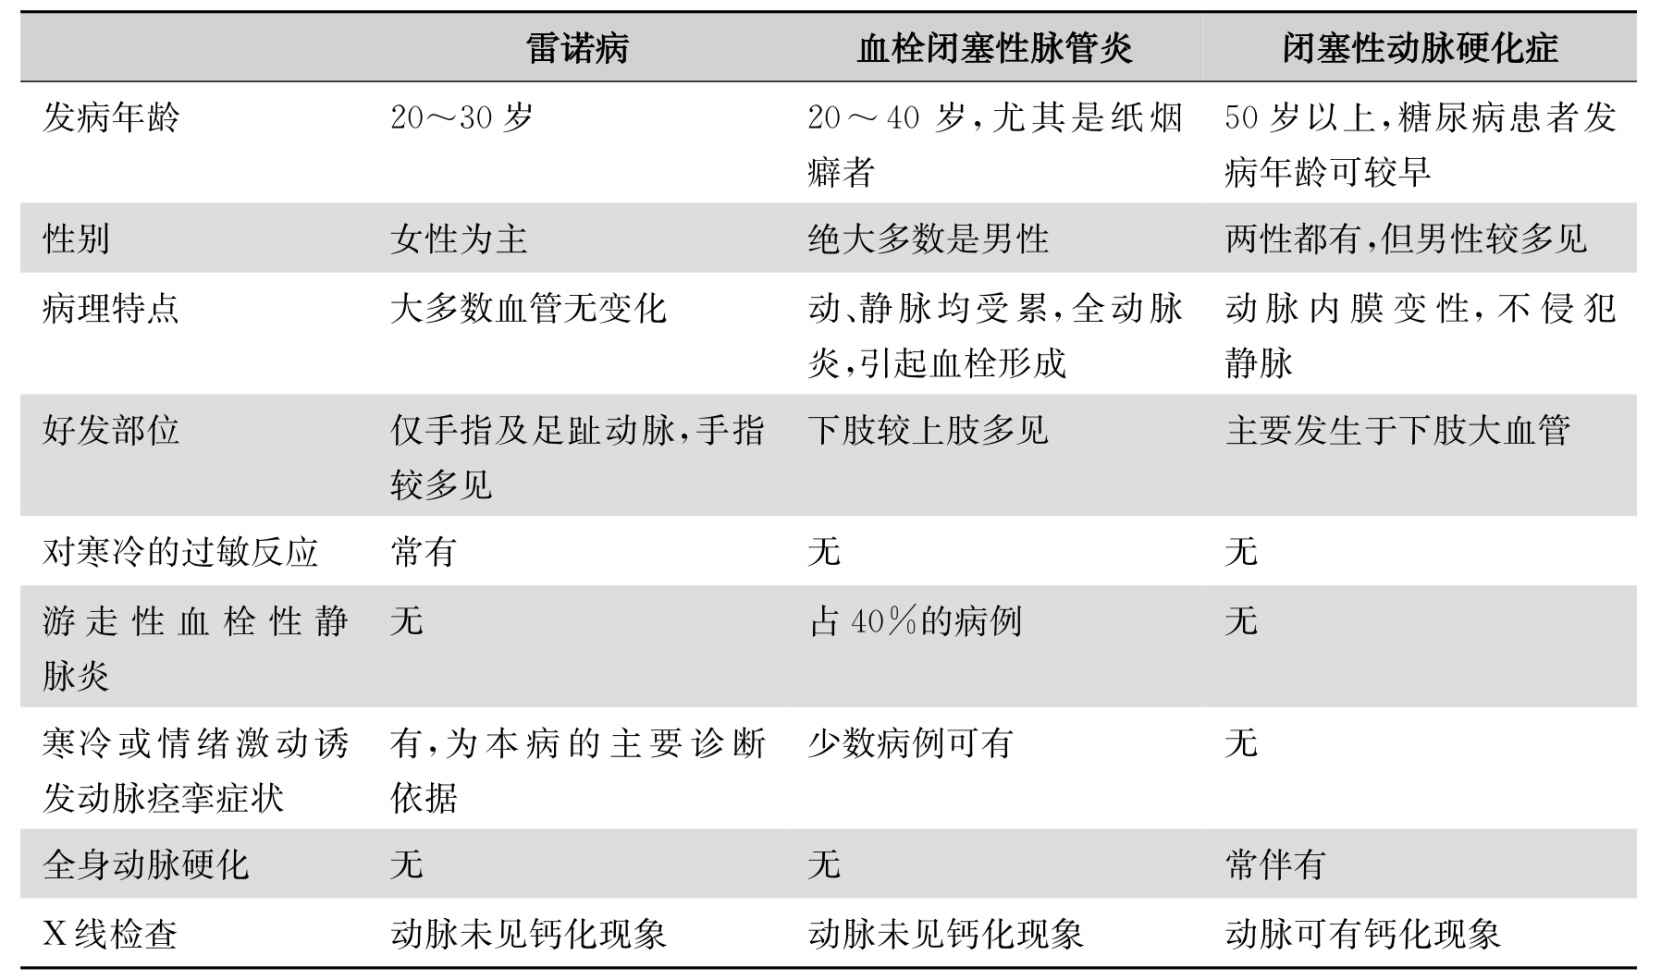
\includegraphics[width=5.97917in,height=3.52083in]{./images/Image00274.jpg}
\end{table}

\subsubsection{(二)红斑性肢痛}

本病的主要症状是患者的肢端(有时只有一个或两个趾或指)阵发性血管扩张、发红、皮肤温度升高,疼痛剧烈。本病国内有不少病例报告。发病机制尚未清楚。过去教科书记载多见于青年男性。广州地区报告433例中,青年女性最多,占92.86\%。起病较急,主要是双足同时发病,少数也累及双手。当患者局部温度超过一定的临界温度(约在33~34℃)时,疼痛立即发生,而低于此界限则疼痛消失。疼痛多为烧灼样,有些表现为刺痛或胀痛,症状夜间比白昼重。热刺激、行动及足垂吊姿势均可使疼痛加剧;浸冷水、抬高患肢或将足露出被外,均可使疼痛暂时缓解。疼痛时患部有潮红充血现象,局部皮肤温度升高(达35~37℃),伴有出汗、足背动脉与胫后动脉搏动增强,故与血栓闭塞性脉管炎有所不同。患者全身情况良好,发作间歇期肢端仍常遗留轻度麻木感与轻度疼痛,但不伴发神经营养障碍如溃疡和坏疽等。

除上述的原发性红斑性肢痛外,继发性红斑性肢痛可见于真性红细胞增多症、糖尿病等。

\protect\hypertarget{text00342.html}{}{}

\section{151 骨与关节及关节周围组织疾病}

参见第42、43章。

\protect\hypertarget{text00343.html}{}{}

\section{152 骨疾病}

由于骨疾病引起的肢痛,较起源于其他疾病者少见。但骨疾病早期易被漏诊。X线、CT、MR等影像学检查是重要的诊断方法。

\subsection{一、骨质疏松、骨质软化(参见第39章)}

\subsection{二、骨肿瘤、骨炎、骨坏死、骨折}

骨肿瘤、骨炎、骨梅毒、骨结核、骨雅司、骨髓炎、骨膜炎、骨无菌性坏死、骨折等均可引起不同程度的患肢局部疼痛,影像学检查有重要的诊断意义。

\subsection{三、骨膜下出血}

本病可见于血友病、维生素C缺乏症、血小板减少性紫癜等出血性疾病;主要症状为受累骨的局部疼痛,触诊有硬块,常伴有皮下及黏膜出血。本病的诊断必须找出其原发病而确定之。

\subsection{四、骨嗜酸性肉芽肿}

骨嗜酸性肉芽肿国内有多例报告。本病是组织细胞病X的特别良性类型。骨病变可为局限性或多发性。好发于扁平骨,少见于长骨,受累骨按好发程度排列,依次为肋骨、颅骨、椎体、股骨、下颌骨和肱骨。半数以上病变累及下肢骨、肋骨和颅骨。

本病主要累及青少年,单发性病变者常无全身症状,仅表现为局部较轻疼痛、肿胀和压痛;多发性病变者疼痛较剧烈。大多数患者以患肢疼痛、跛行为主诉而就诊。可伴有发热、食欲减退、消瘦等全身症状。四肢病变偶可引起病理性骨折。颅骨病变表现为凹陷畸形;脊柱病变有时可引起臂丛神经受压,出现上肢放射性疼痛和感觉障碍。

本病的血象可有轻度嗜酸性粒细胞增多(偶达10\%以上),血清碱性磷酸酶增高,骨髓检查可见嗜酸性粒细胞增多。诊断主要根据骨活检。

\subsection{五、畸形性骨炎(Paget病)}

本病是一种原因未明的慢性进行性骨病,国内有少数病例报告。约1/4的病例无症状。常见症状为骨疼痛与畸形。患者多因患部疼痛、畸形而就诊。有时因骨折或恶性变(发生率2\%~10\%)等并发症而就诊。本病可发生于一骨的一部分,一般均超过一半以上,也可同时侵犯数骨。国内报告病例有侵犯股骨、颅骨、腓骨、胫骨、肱骨等。血液化学检查血清钙、磷值一般正常,但血清碱性磷酸酶则有明显增高,可高达正常值的4~5倍。尿及粪中钙、磷排量也不增加。X线检查早期表现为急性脱钙,无特征性;晚期则极为典型,可分为三型:骨松变型、骨硬化型与骨硬化囊肿型,其中以骨松变型最为常见。累及颅骨时,可出现头颅增大、听力减退、面肌痉挛等症状。如发生恶性变,受累部位有不规则的骨破坏或放射状骨刺形成,局部一般也有软组织肿块出现,同时疼痛加剧,局部病变进行加速。

\subsection{六、跟痛症}

据国内作者107例跟痛症的研究报道,患者以中年女性多见,40~60岁为高发年龄组。跟痛症可能与体内激素代谢水平有关。疼痛侧足跟腱组织肿胀,提示跟痛症与足跟腱组织炎症有关,而与跟骨骨刺的大小、方向及形状无关。临床上也观察到有跟痛症的患者不一定有骨刺,而有骨刺的足跟不一定有疼痛。此组患者经局部按摩理疗及局部泼尼松龙液注射治疗,2周左右奏效。

\protect\hypertarget{text00344.html}{}{}

\section{153 四肢肌肉疾病}

\subsection{一、痛性痉挛}

痛性痉挛是一种疼痛性肌肉强直性收缩,可发生于任何年龄,但以老年人及孕妇多见。最常受累者为腓肠肌,发作多在夜间、过度活动或受凉后。发作时腓肠肌突然绷紧、坚硬、挛缩性疼痛。持续几秒乃至数十秒方缓解。

\subsection{二、手足搐搦症}

手足搐搦症以疼痛性、痉挛性肌肉收缩为特征,常伴有麻木、感觉异常和疼痛。发作时可出现上臂内收肘屈曲,腕及指屈曲,呈握拳状,或指间关节伸直、大拇指内收,在下肢双足呈内翻尖足位,膝关节及髋关节屈曲。严重者全身骨骼肌与平滑肌均可呈痉挛状态,可发生喉、气管、胃肠、膀胱、膈甚至心肌痉挛。手足搐搦症最常见于低钙血症,但血钙总量正常而有碱中毒时也可发生本症。

\subsection{三、炎性肌病}

炎性肌病主要包括多发性肌炎和皮肌炎。多发性肌炎的典型症状是对称性的近端肢体无力(肩胛带、骨盆带肌受累所致),肌肉酸痛并有压痛,严重者出现肌萎缩,小部分患者亦可有远端肢体无力和肌肉酸痛,多无感觉障碍,可伴有发热和吞咽困难。血清肌酶(包括肌酸激酶、谷草转氨酶等)检测、肌电图、肌活检等检查对诊断的确立具有重要价值。多发性肌炎患者如出现Gottron征、眼睑和胸上部等处的紫红色皮症、技工手等特征性皮疹时则应诊断为皮肌炎。

\subsection{四、风湿性多肌痛}

本病是一种以四肢近端和躯干疼痛为特征的综合征,主要表现为肩、骨盆带肌颈部等部位的疼痛和僵硬,症状有时和多发性肌炎非常相似,但血清肌酶正常,多见于50岁以上患者,血沉升高,小剂量糖皮质激素反应迅速有效。

\subsection{五、其他原因的肌痛}

\subsubsection{(一)钩端螺旋体病}

本病常引起剧烈肌痛,尤以腓肠肌痛最为显著。中山大学附属第一医院报告的一组病例中,约2/3的病例有腓肠肌压痛,且早期出现,也为提示诊断此病的重要线索。诊断参见第3.1.6节。

\subsubsection{(二)人旋毛虫病}

本病因摄食半熟肉或生肉感染旋毛虫所引起。近年国内有不少病例报告,常引起全身肌肉酸痛,尤以腓肠肌为甚,伴明显压痛,重者稍触摸皮肤也感疼痛。肌肉疼痛常持续三周以上,甚至长达两个月;且伴四肢乏力、发热,早期出现凹陷性水肿、皮肤瘙痒等症状。患者血中常有显著的嗜酸性粒细胞增多,据文献报道,血嗜酸性粒细胞增多高达20\%~75\%以上。肌活检有助于确诊。

\subsubsection{(三)维生素C缺乏症}

本病可引起肌肉出血,往往早期引起下肢肿痛、肌肉僵硬,不能站立,触诊也有明显的压痛。患者一般同时有皮肤、牙龈和口腔黏膜出血。

\subsubsection{(四)热痉挛}

本病主要发生于高温下作业的工人,肌肉痉挛与大量丢失氯化钠有关。患者主诉乏力、口渴、肌痉挛及疼痛,尤以腓肠肌、腹直肌等为明显。

\subsubsection{(五)职业性肌痉挛}

本病乃因某些手艺操作,手指活动频繁,疲劳过度,以至引起手部肌肉痉挛性疼痛,可见于打字员、打电报员、挤奶员、抄写员、乐器演奏者等。体检时无神经肌肉病征,停止这些操作后不再出现痉挛。

\subsubsection{(六)横纹肌血管瘤}

本病是肌肉内血管组织的先天性异常或畸形,也称血管错构瘤,国内有少数病例报告。此瘤多发生于四肢肌肉,主要症状为局部肿胀,皮肤温度稍增高,有疼痛和压痛,肢体活动时疼痛加剧,有的患者由于肿物不断增大,影响肢体活动,肌肉发生失用性萎缩,甚至肢体畸形和残废。有时在肿物之上触到搏动和听到血管杂音。本病病程经过缓慢,患者全身情况良好,局部穿刺抽出血液可确定诊断。X线检查受累肌肉或其他非正常的静脉丛可发现静脉石,此为血管瘤的特殊X线征。最有确诊价值的方法是局部直接注入35\%造影剂4~20ml,进行肿物内直接造影。

\subsubsection{(七)药物诱导性肌病}

临床上常用的许多药物如糖皮质激素、他汀类药物、阿司匹林、羟基氯喹、普鲁卡因胺等均可引起四肢肌肉疼痛、无力等表现。这类肌病易被忽视,而一旦发现又较容易治疗,所以寻找肌痛的原因时要想到这类疾病。

\subsubsection{(八)遗传性异常引起的肌病}

糖原累积病、线粒体肌病等遗传性疾病亦可出现运动后肌肉疼痛、肌无力、肌萎缩等表现,但常有原发病的表现可资鉴别。

\protect\hypertarget{text00345.html}{}{}

\section{参考文献}

1.沈伯台,等.红斑肢痛症233例报告.中华医学杂志,1984,64:49

2.周墨宽,勇强.多普勒超声诊断下肢静脉血栓形成.中华外科杂志,1991,29(2):113-115

3.张强,段志泉.超声血管造影用于诊断周围血管疾病.中华外科杂志,1995,33(7):422-424

4.赵春起,等.下肢动脉闭塞症疾病多普勒波形的临床分析.中华外科杂志,1988,36:6

5.周方,党耕町.神经源性间歇性跛行的病因分析.中华外科杂志,1995,33(3):140-143

6.第二届颈椎病专题座谈会纪要.中华外科杂志,1993,31(8):472-476

7.吕厚山,谷国良.跟痛症与跟骨结节骨赘.中华外科杂志,1996,34(5):294-296

8.吴志全,蒋小平.Parkes-Weber综合征五例报告.中华外科杂志,1993,31(12):749-751

9.廖琳,徐德凤.糖尿病下肢血管病变的彩色多普勒检查及治疗.中华内分泌代谢杂志,1996,12(3):186-187

10.卢祖能,汤晓芙.腕管综合征262例的回顾性分析.中华神经科杂志,1996,29(2):115-118

11.吴东海.多发性肌炎和皮肌炎//蒋明,等.中华风湿病学.北京:华夏出版社,2004:1091-1105

12.张奉春,等.巨细胞动脉炎和风湿性多肌痛//蒋明,张奉春.风湿病诊断与诊断评析.上海:上海科学技术出版社,2004:281-287

\protect\hypertarget{text00346.html}{}{}

